\chapter{Heaps}
\chaplabel{heaps}

Neste capítulo, discutiremos duas implementações da estrutura de dados de prioridade #Fila# extremamente útil. Ambas as estruturas são um tipo especial de árvore binária chamada \emph{heap},
\index{heap}%
\index{binary heap}%
\index{heap!binary}%
o que significa ``uma pilha desorganizada.'' Isso contrasta com as árvores de busca binária que podem ser consideradas como uma pilha altamente organizada.

A primeira implementação de \textit{heap} usa um array para simular uma árvore binária completa. Esta implementação muito rápida é a base de um dos mais rápidos algoritmos de ordenação conhecidos, o chamado \textit{heapsort} (ver \secref{heapsort}).
A segunda implementação é baseada em árvores binárias mais flexíveis.
Ela suporta uma operação #meld(h)# que permite que a fila de prioridades absorva os elementos de uma segunda fila de prioridade #h#.

\section{#BinaryHeap#: Uma árvore binária implícita}
\seclabel{binaryheap}

\index{BinaryHeap@#BinaryHeap#}%
Nossa primeira implementação de uma  #Fila# (de prioridade) é baseada em uma técnica que tem mais de quatrocentos anos de idade.  O \emph{método Eytzinger}
\index{Eytzinger's method}%
nos permite representar uma árvore binária completa como um array, colocando os nós da árvore em ordem de largura
(ver \secref{bintree:traversal}).
Desta forma, a raiz é armazenada na posição 0, o filho esquerdo da raiz é armazenado na posição 1, o filho direito da raiz na posição 2, o filho esquerdo do filho esquerdo da raiz é armazenado na posição 3 e assim por diante.
Ver \figref{eytzinger}.

\begin{figure}
  \begin{center}
    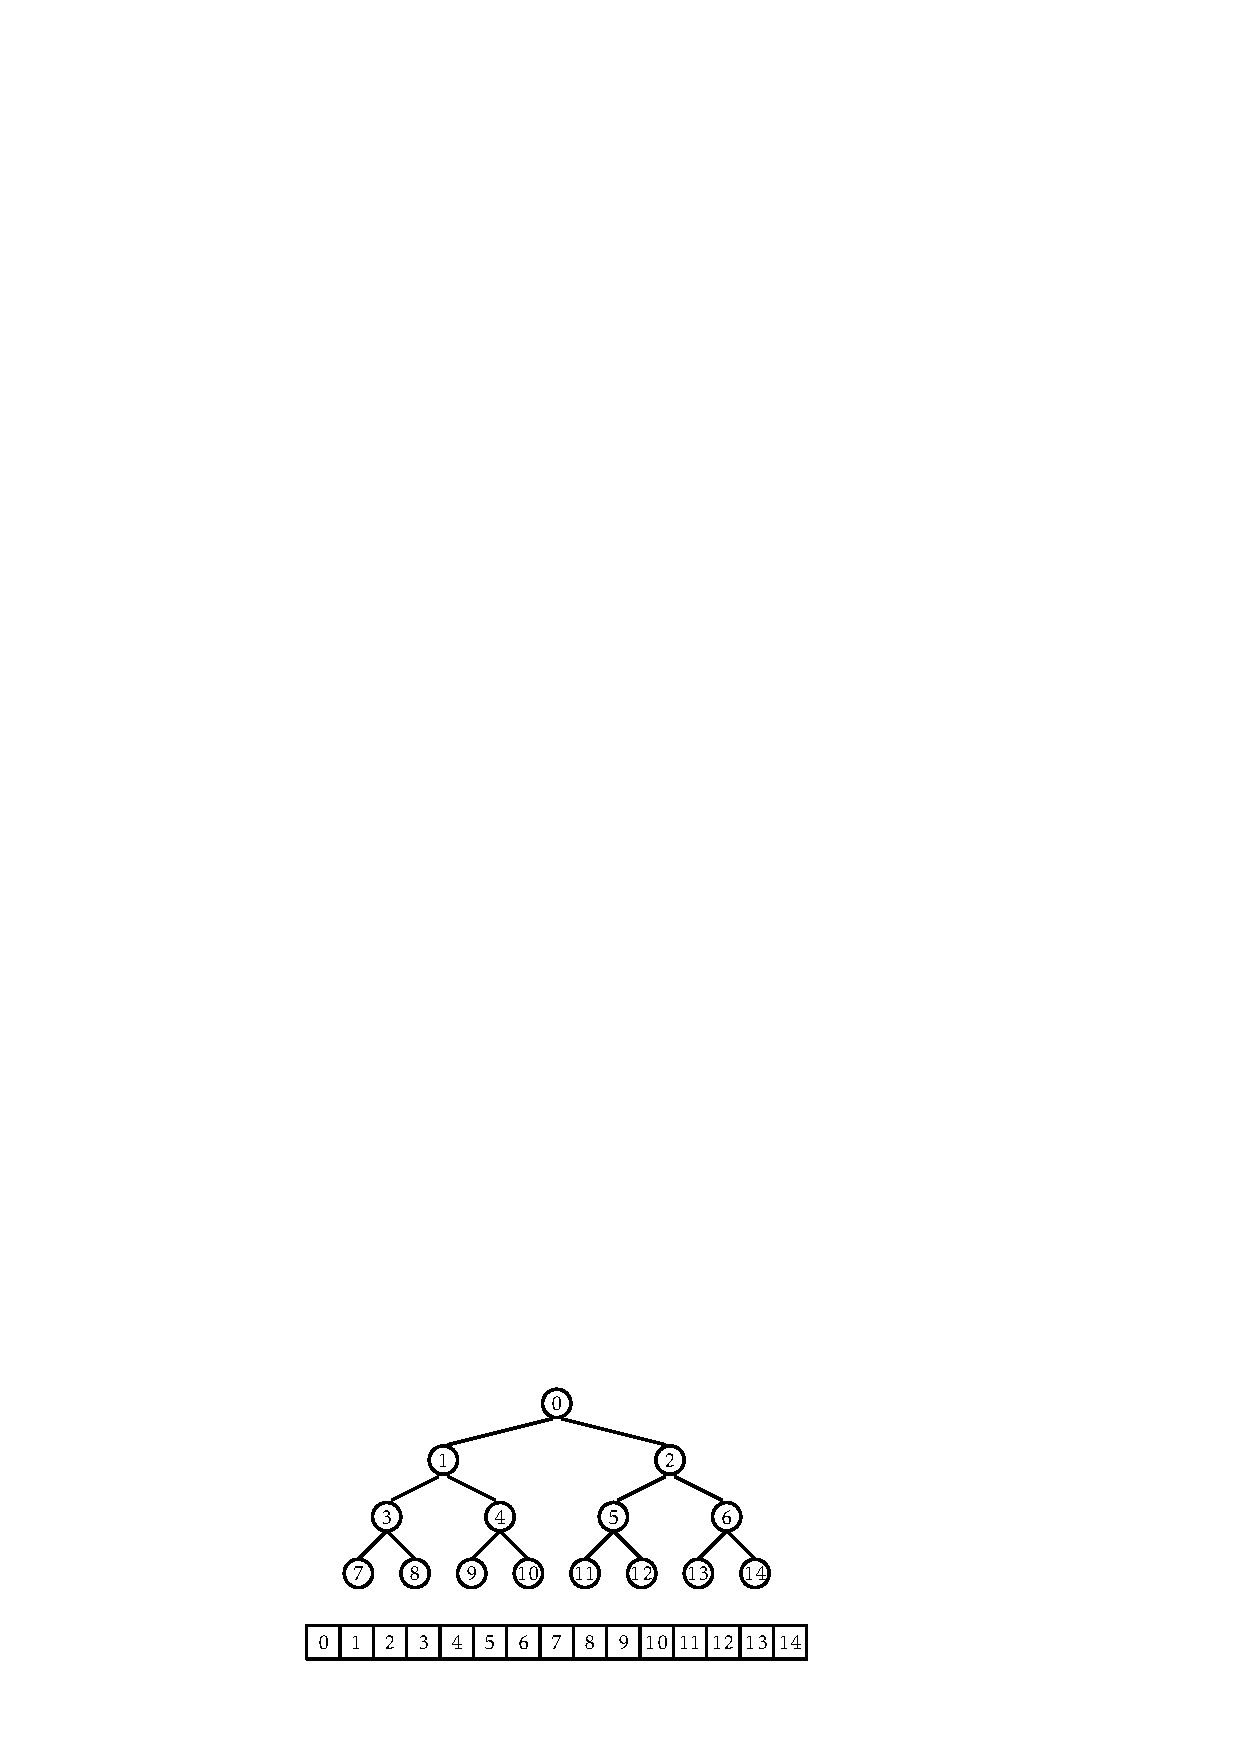
\includegraphics[scale=0.90909]{figs/eytzinger}
  \end{center}
  \caption{O método de Eytzinger representa uma árvore binária completa como um array.}
  \figlabel{eytzinger}
\end{figure}

Se aplicarmos o método de \textit{Eytzinger} a uma árvore suficientemente grande, alguns padrões surgem. O filho esquerdo do nó no índice #i# está no índice $#left(i)#=2#i#+1$ e o filho direito do nó no índice #i# está no índice $#right(i)#=2#i#+2$. O pai do nó no índice #i# está no índice $#parent(i)#=(#i#-1)/2$.
\codeimport{ods/BinaryHeap.left(i).right(i).parent(i)}

Uma #BinaryHeap# usa essa técnica para representar implicitamente uma
árvore binária em que os elementos são \emph{ordenados pelo heap}:
\index{heap-ordered binary tree}%
\index{binary tree!heap-ordered}%
\index{heap order}%
o valor armazenado em qualquer índice #i# não é menor que o valor armazenado no índice #parent(i)#, com a exceção do valor da raiz, $#i#=0$. Segue-se que o menor valor na #Fila# de prioridade é, portanto, armazenado na posição 0 (a raiz).

Na #BinaryHeap#, os #n# elementos são armazenados em um array #a#:
\codeimport{ods/BinaryHeap.a.n}

Implementar a operação #add(x)# é bastante simples. Como acontece com todas as estruturas baseadas em array, primeiro verificamos se #a# está cheio (verificando se $#a.length#=#n#$) e, em caso afirmativo, aumentamos #a#. Em seguida, colocamos #x# no local #a[n]# e incrementamos #n#. Neste ponto, tudo o que resta é garantir que mantemos a propriedade do \textit{heap}. Fazemos isso trocando repetidamente #x# por seu pai até que #x# não seja menor que seu pai.
Ver \figref{heap-insert}.
\codeimport{ods/BinaryHeap.add(x).bubbleUp(i)}

\begin{figure}
  \begin{center}
    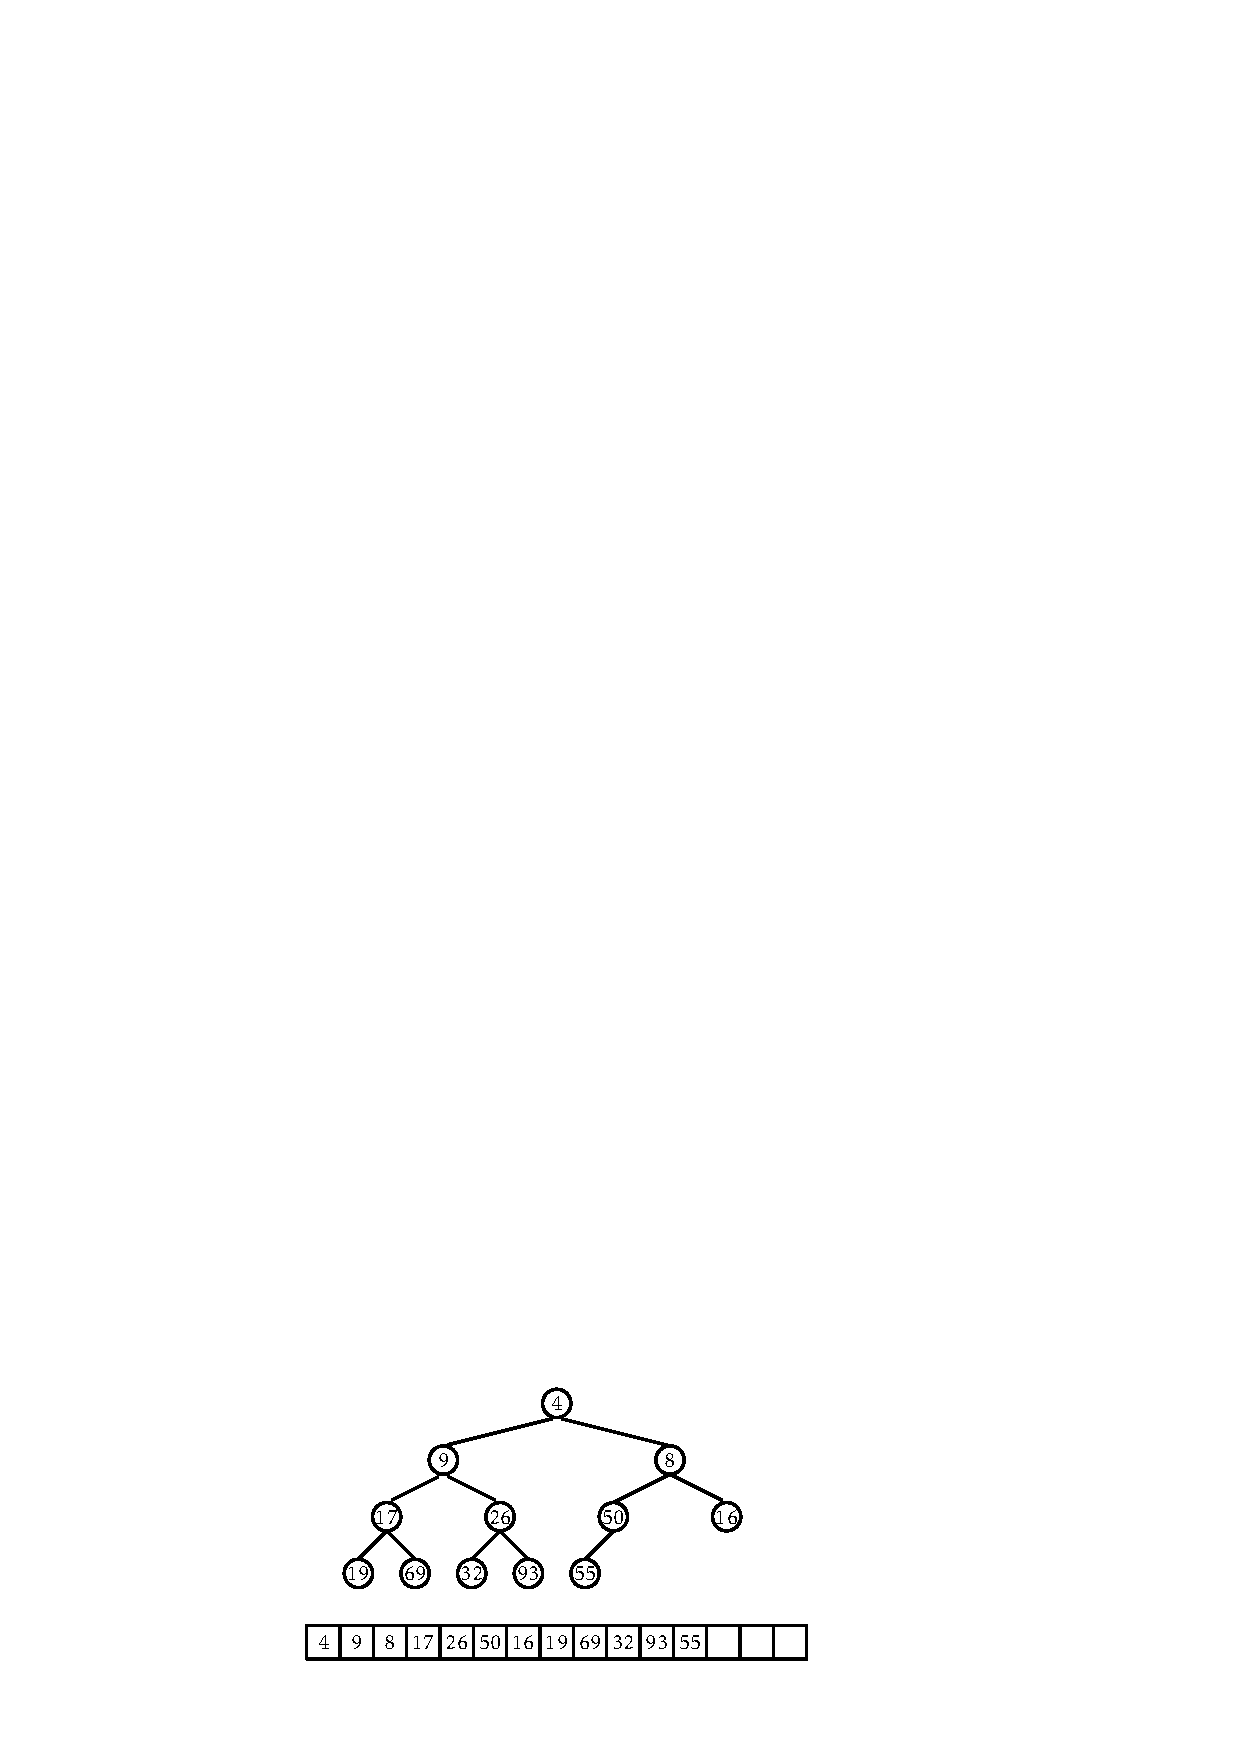
\includegraphics[height=\QuarterHeightScaleIfNeeded]{figs/heap-insert-1} \\
    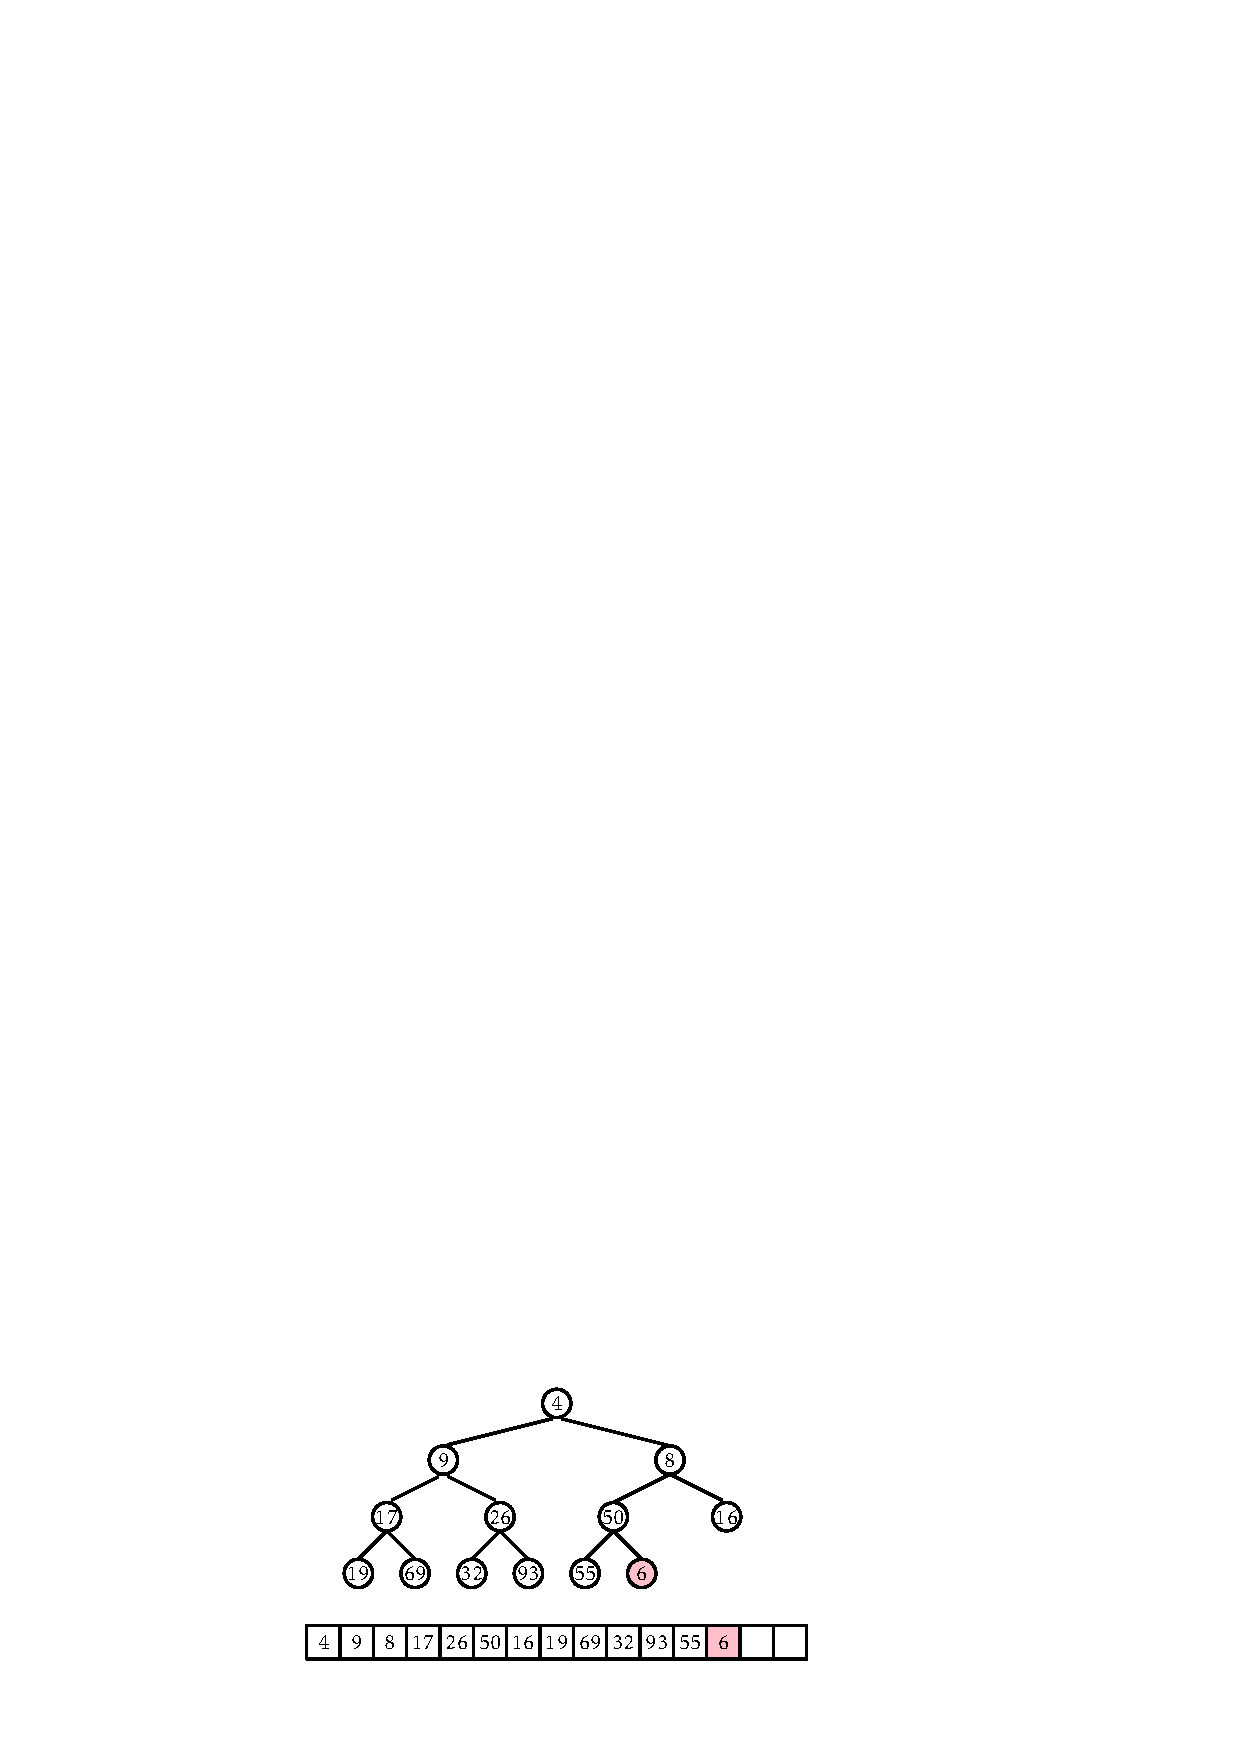
\includegraphics[height=\QuarterHeightScaleIfNeeded]{figs/heap-insert-2} \\
    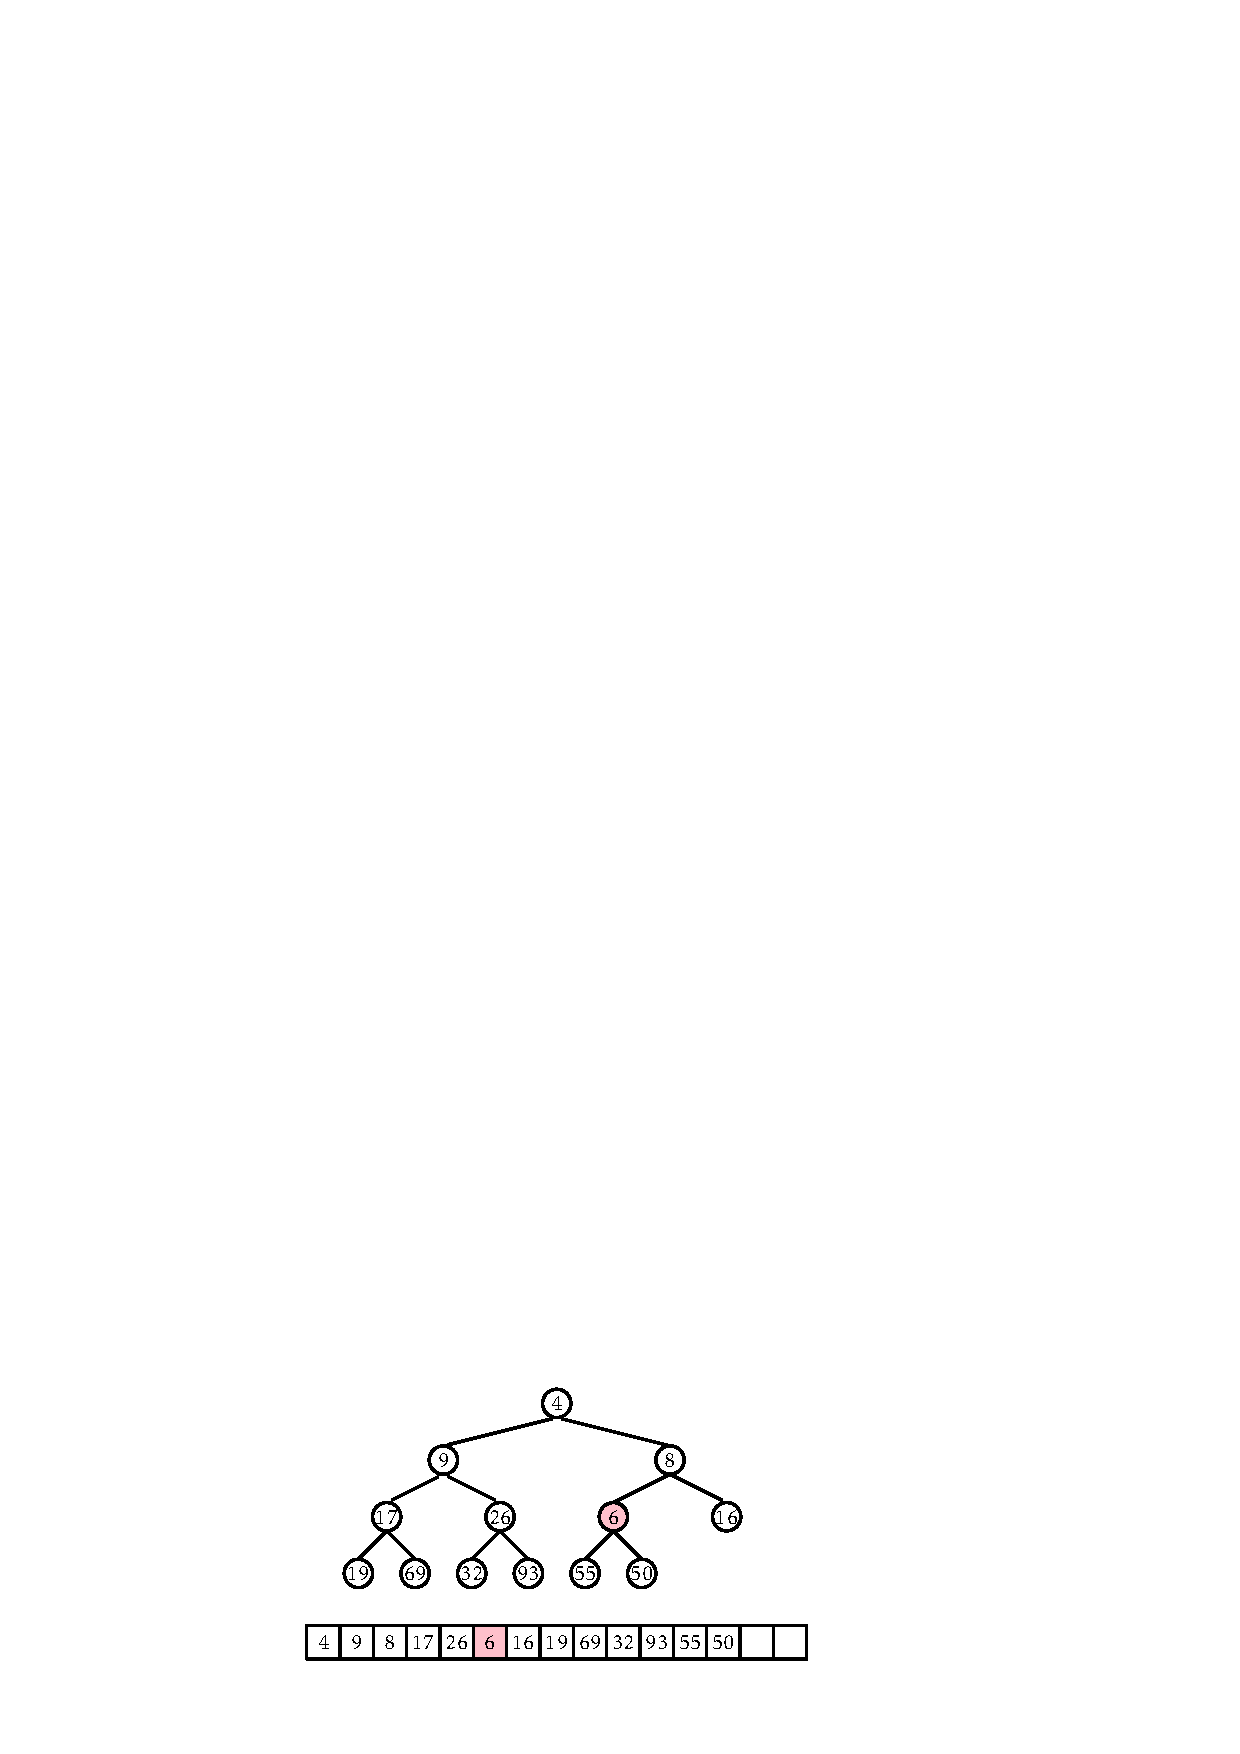
\includegraphics[height=\QuarterHeightScaleIfNeeded]{figs/heap-insert-3} \\
    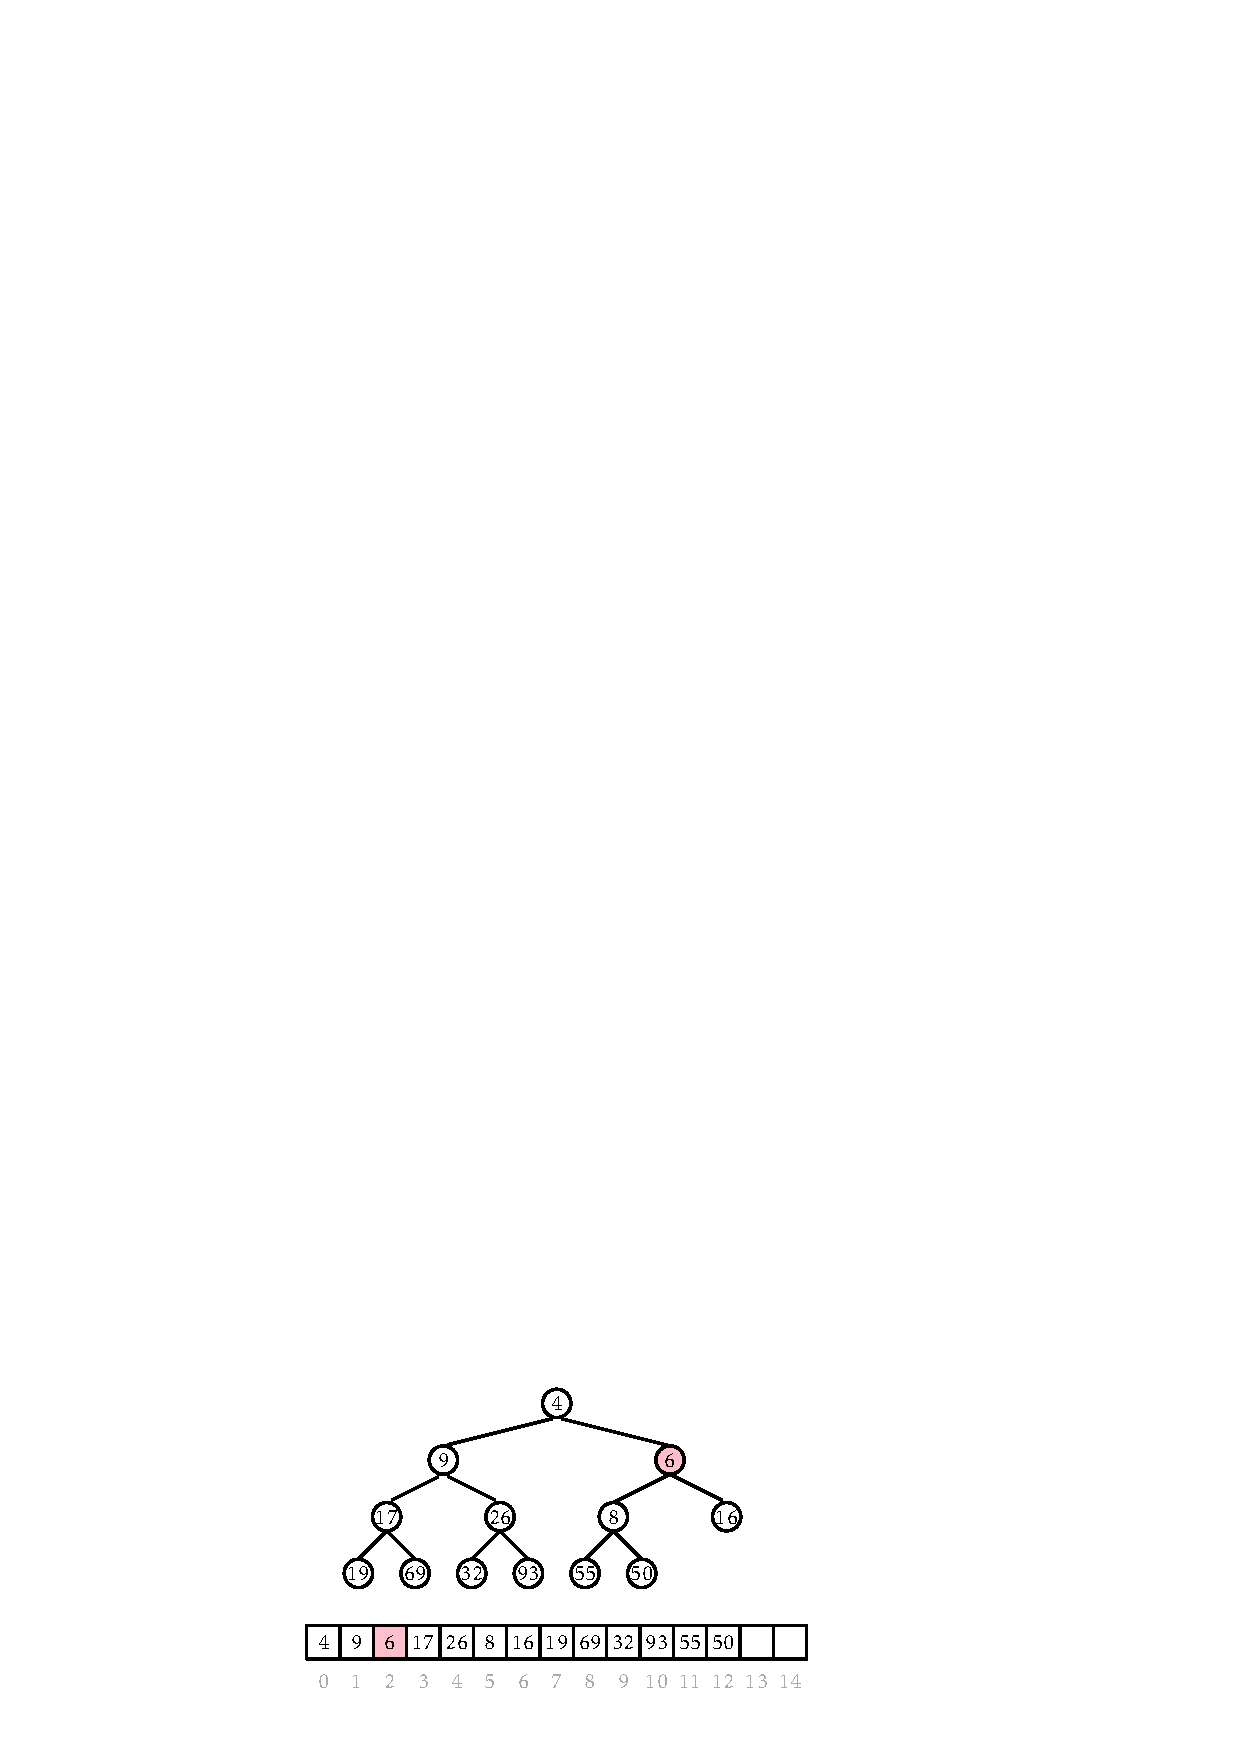
\includegraphics[height=\QuarterHeightScaleIfNeeded]{figs/heap-insert-4} \\
  \end{center}
  \caption[Adicionando a um BinaryHeap] {Adicionando o valor 6 à #BinaryHeap#.}
  \figlabel{heap-insert}
\end{figure}

Implementar a operação #remove()#, que remove o menor valor do \textit{heap}, é um pouco mais complicado. Nós sabemos onde o menor valor está (na raiz), mas precisamos substituí-lo depois de removê-lo e garantir que mantemos a propriedade de \textit{heap}.

A maneira mais fácil de fazer isso é substituir a raiz pelo valor #a[n-1]#, excluir esse valor e decrementar #n#. Infelizmente, o novo elemento raiz agora provavelmente não é o menor elemento, por isso ele precisa ser movido para baixo.
Fazemos isso comparando repetidamente esse elemento com seus dois filhos.
Se é o menor dos três, então estamos prontos. Caso contrário, nós trocamos este elemento pelo menor de seus dois filhos e continuamos.
\codeimport{ods/BinaryHeap.remove().trickleDown(i)}

\begin{figure}
  \begin{center}
    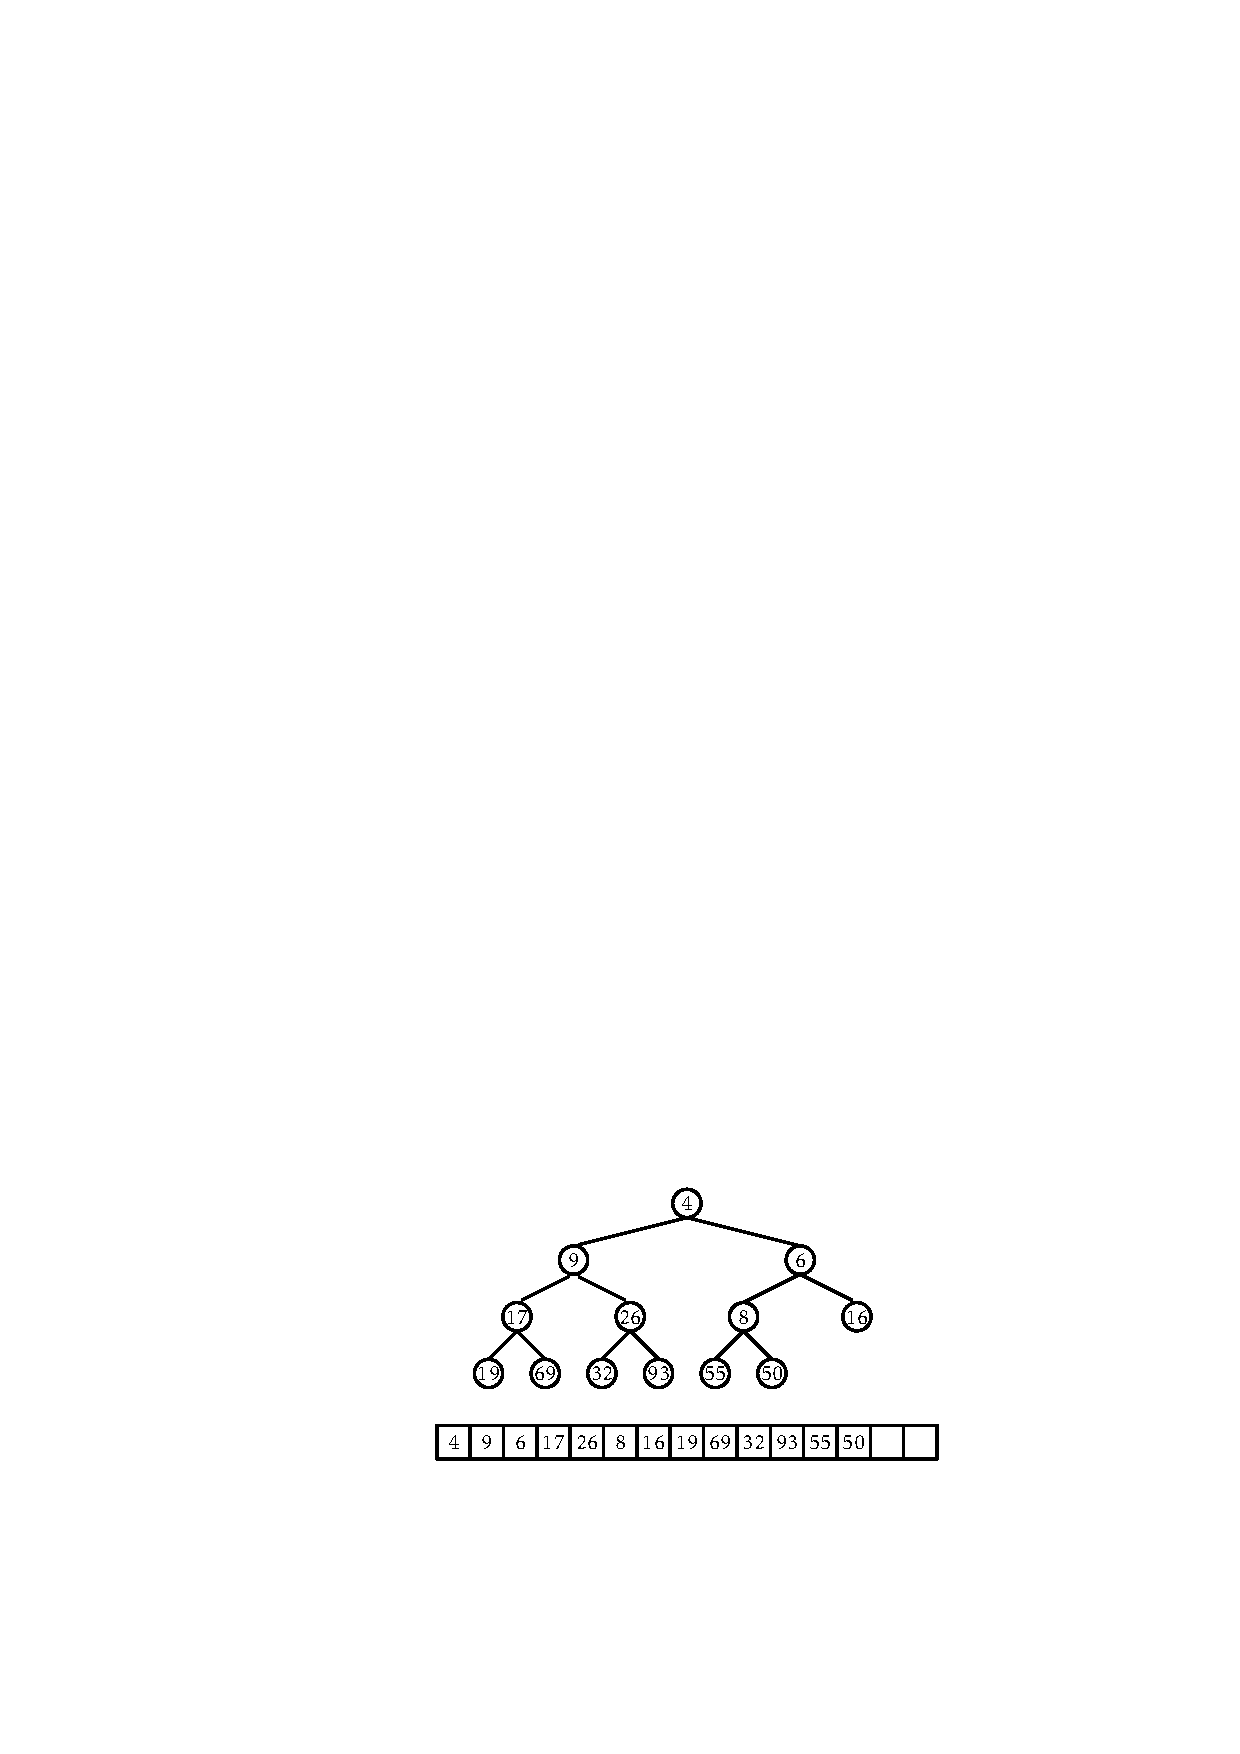
\includegraphics[height=\QuarterHeightScaleIfNeeded]{figs/heap-remove-1} \\
    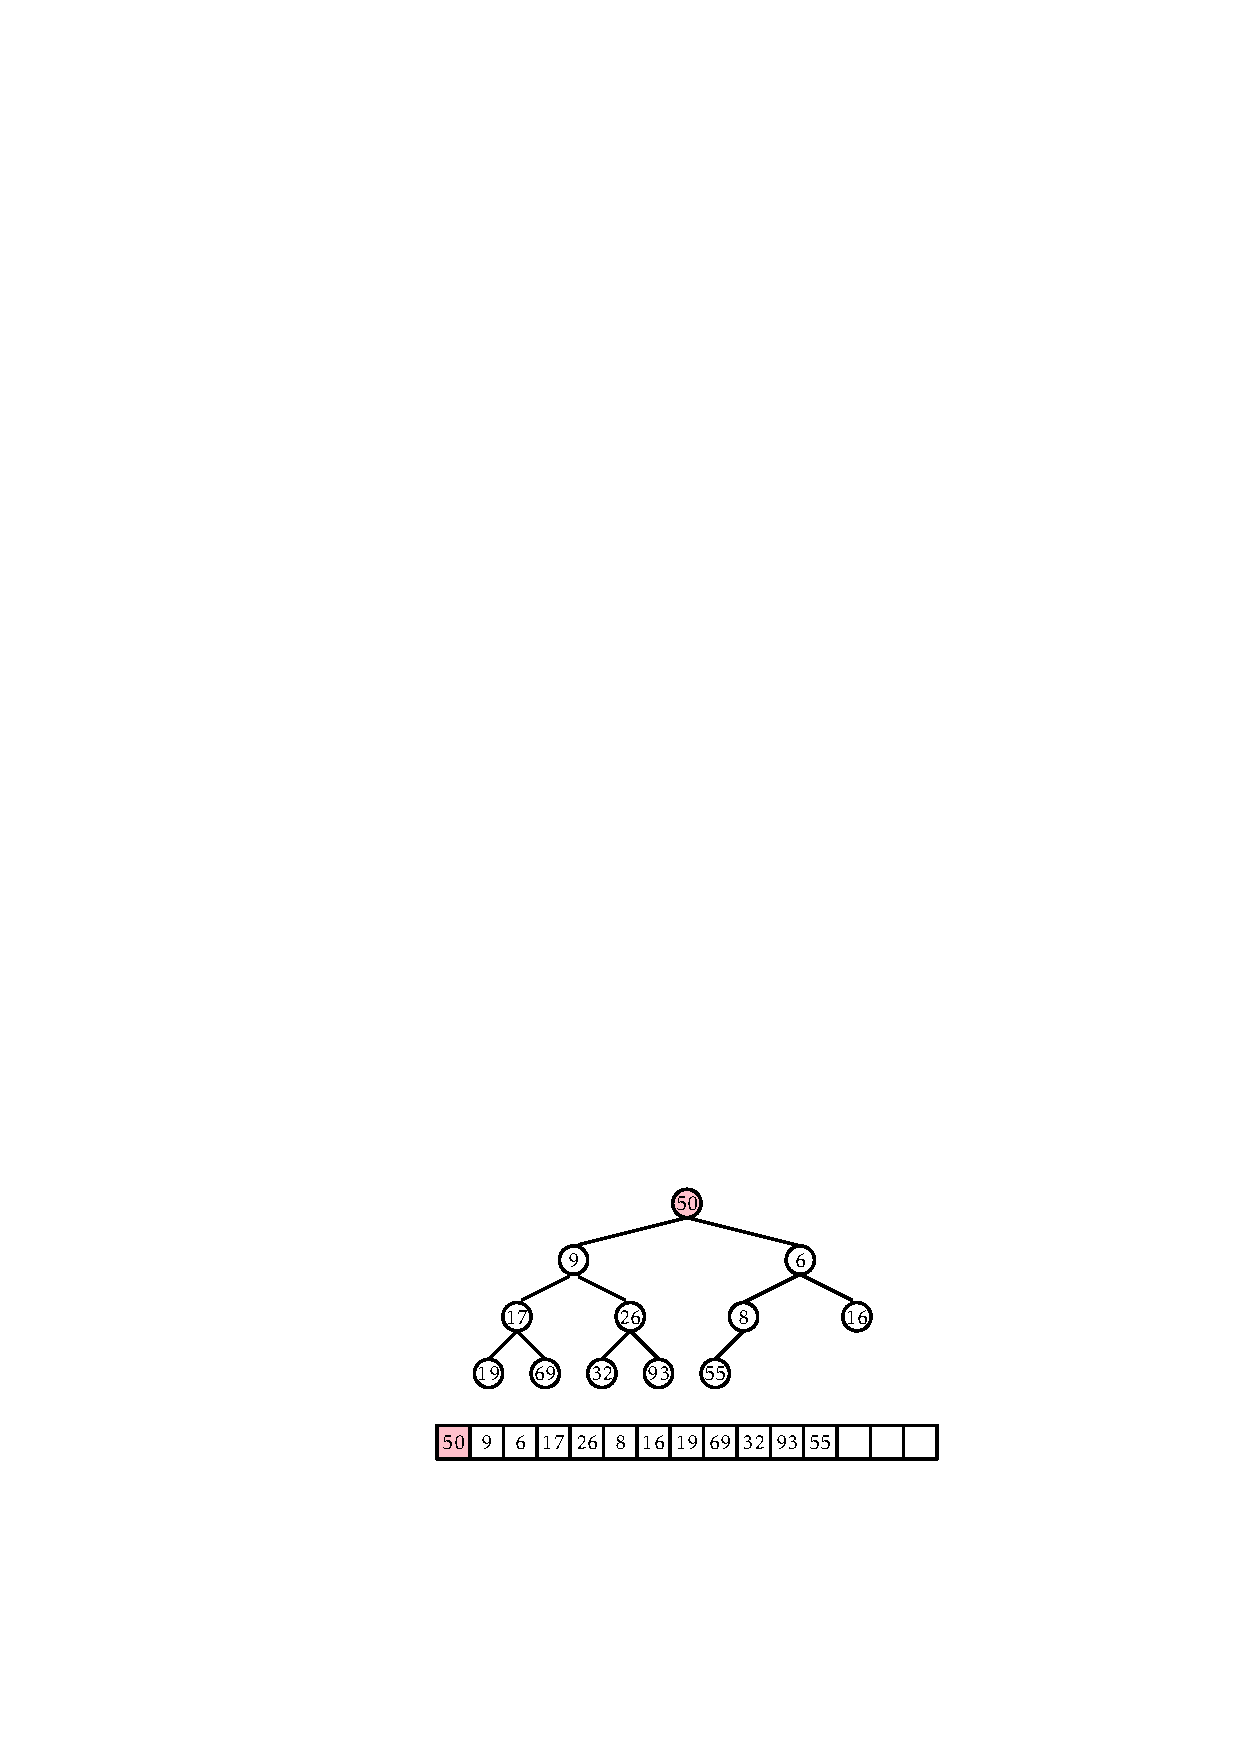
\includegraphics[height=\QuarterHeightScaleIfNeeded]{figs/heap-remove-2} \\
    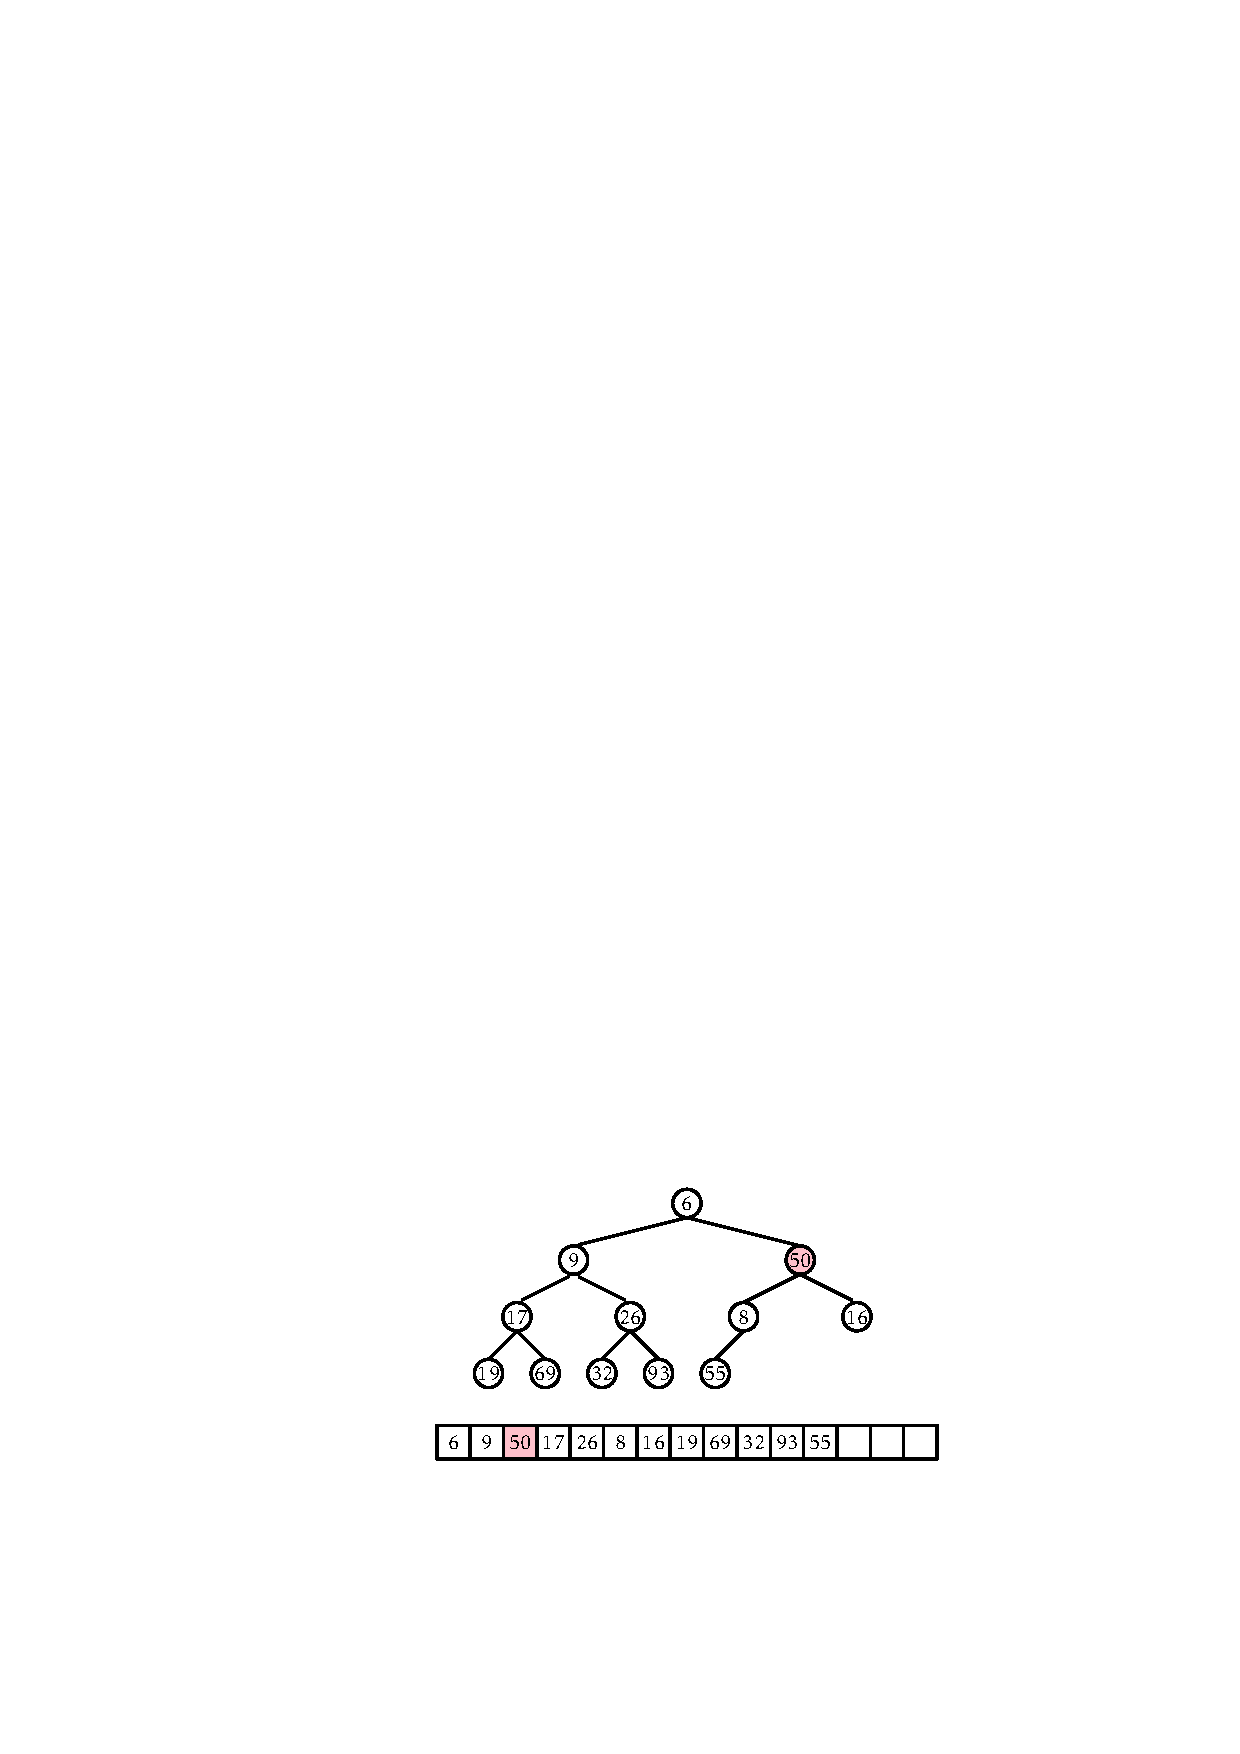
\includegraphics[height=\QuarterHeightScaleIfNeeded]{figs/heap-remove-3} \\
    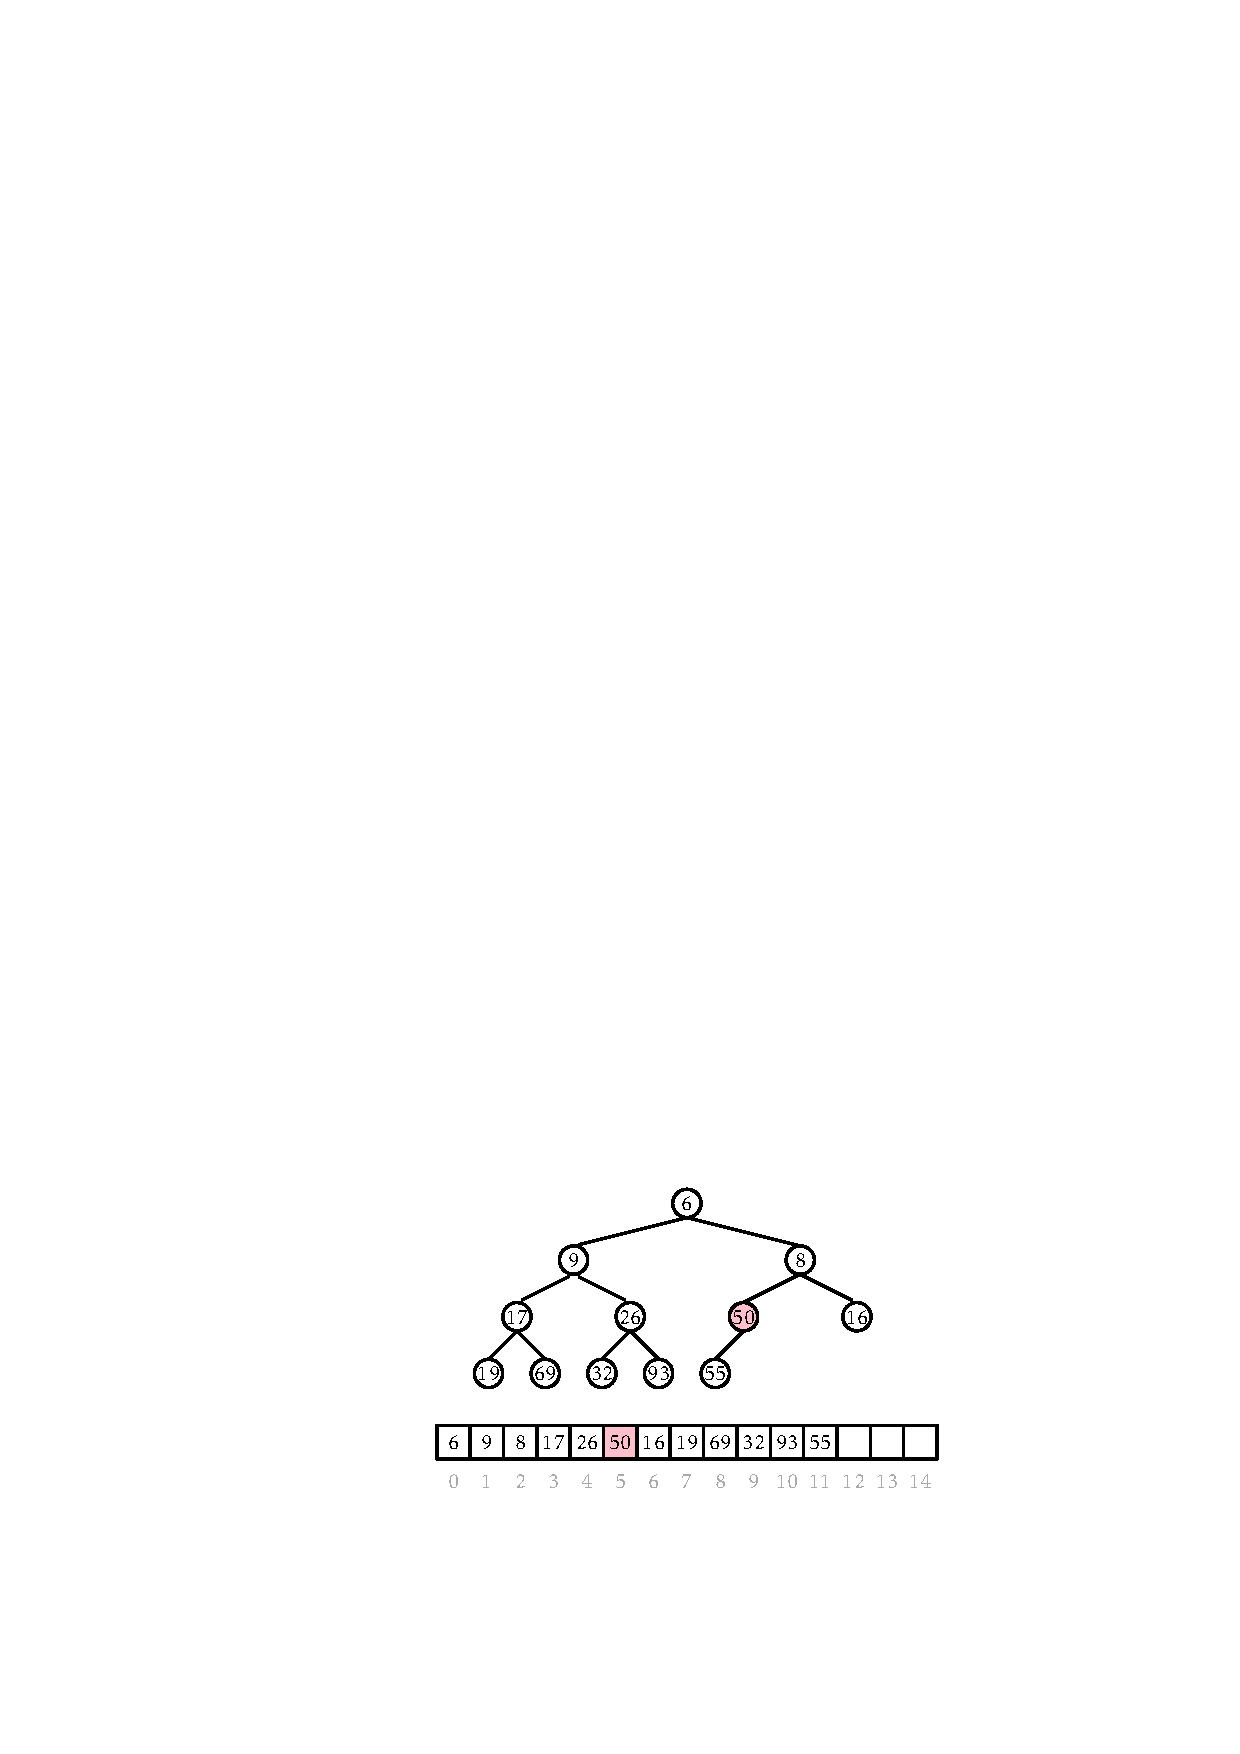
\includegraphics[height=\QuarterHeightScaleIfNeeded]{figs/heap-remove-4} \\
  \end{center}
  \caption[Removendo de uma BinaryHeap]{Removendo o valor mínimo, 4, de uma #BinaryHeap#.}
  \figlabel{heap-remove}
\end{figure}


Como com outras estruturas baseadas em array, iremos ignorar o tempo gasto em chamadas para #resize()#, uma vez que elas podem ser contabilizadas usando o argumento de amortização do \lemref{arraystack-amortized}. Os tempos de execução de #add(x)# e #remove()# dependem da altura da árvore binária (implícita). Felizmente, esta é uma árvore binária \emph{completa};
\index{binary tree!complete}% 
\index{complete binary tree}%
cada nível, exceto o último, tem o número máximo possível de nós. Portanto, se a altura dessa árvore for $h$, ela terá pelo menos $2^h$ nós.
\[
  #n# \ge 2^h \enspace .
\]  
Tomando logaritmos em ambos os lados desta equação dá
\[
   h \le \log #n# \enspace .
\]
Portanto, ambas as operações #add(x)# e #remove()# são executadas em um tempo $O(\log #n#)$.

\subsection{Resumo}

O seguinte teorema resume o desempenho de uma #BinaryHeap#:

\begin{thm}\thmlabel{binaryheap}
	Uma #BinaryHeap# implementa a interface  #Fila# (de prioridade).  Ignorando o custo das chamadas para #resize()#, a #BinaryHeap# suporta as operações #add(x)# e #remove()# em um tempo por operação de $O(\log #n#)$.

  Além disso, começando com uma #BinaryHeap# vazia, qualquer sequência de $m$ operações #add(x)# e #remove()# resulta em um total de tempo $O(m)$ gasto durante todas as chamadas para #resize()#.
\end{thm}

\section{#MeldableHeap#: Uma Heap fusionável aleatória}
\seclabel{meldableheap}

\index{MeldableHeap@#MeldableHeap#}%
Nesta seção, descrevemos o #MeldableHeap#, uma implementação da #Fila# de prioridade, na qual a estrutura subjacente também é uma árvore binária ordenada por heap. No entanto, ao contrário de uma #BinaryHeap# no qual a árvore binária subjacente é completamente definida pelo número de elementos, não há restrições quanto à forma da árvore binária subjacente na #MeldableHeap#; qualquer coisa serve.

As operações #add(x)# e #remove()# em uma #MeldableHeap# são
implementadas em termos da operação #merge(h1,h2)#. Essa operação usa dois nós de heap #h1# e #h2# e mescla-os, retornando um nó de heap que é a raiz de uma heap que contém todos os elementos na subárvore com raiz em #h1# e todos os elementos na subárvore com raiz em #h2#.

O bom de uma operação #merge(h1,h2)# é que ela pode ser definida recursivamente. Veja \figref{meldable-merge}. Se #h1# ou #h2# for #nil#, então estamos mesclando com um conjunto vazio, então retornamos #h2# ou #h1#, respectivamente. Caso contrário, assuma $#h1.x# \le #h2.x#$ pois, se $#h1.x# > #h2.x#$, poderemos inverter os papéis de #h1# e #h2#.
Então, sabemos que a raiz da heap mesclada conterá #h1.x# e podemos mesclar recursivamente #h2# com #h1.left# ou #h1.right#, como desejamos.
É aqui que entra a randomização e lançamos uma moeda para decidir se devemos mesclar #h2# com #h1.left# ou #h1.right#:
\codeimport{ods/MeldableHeap.merge(h1,h2)}

\begin{figure}
  \centering{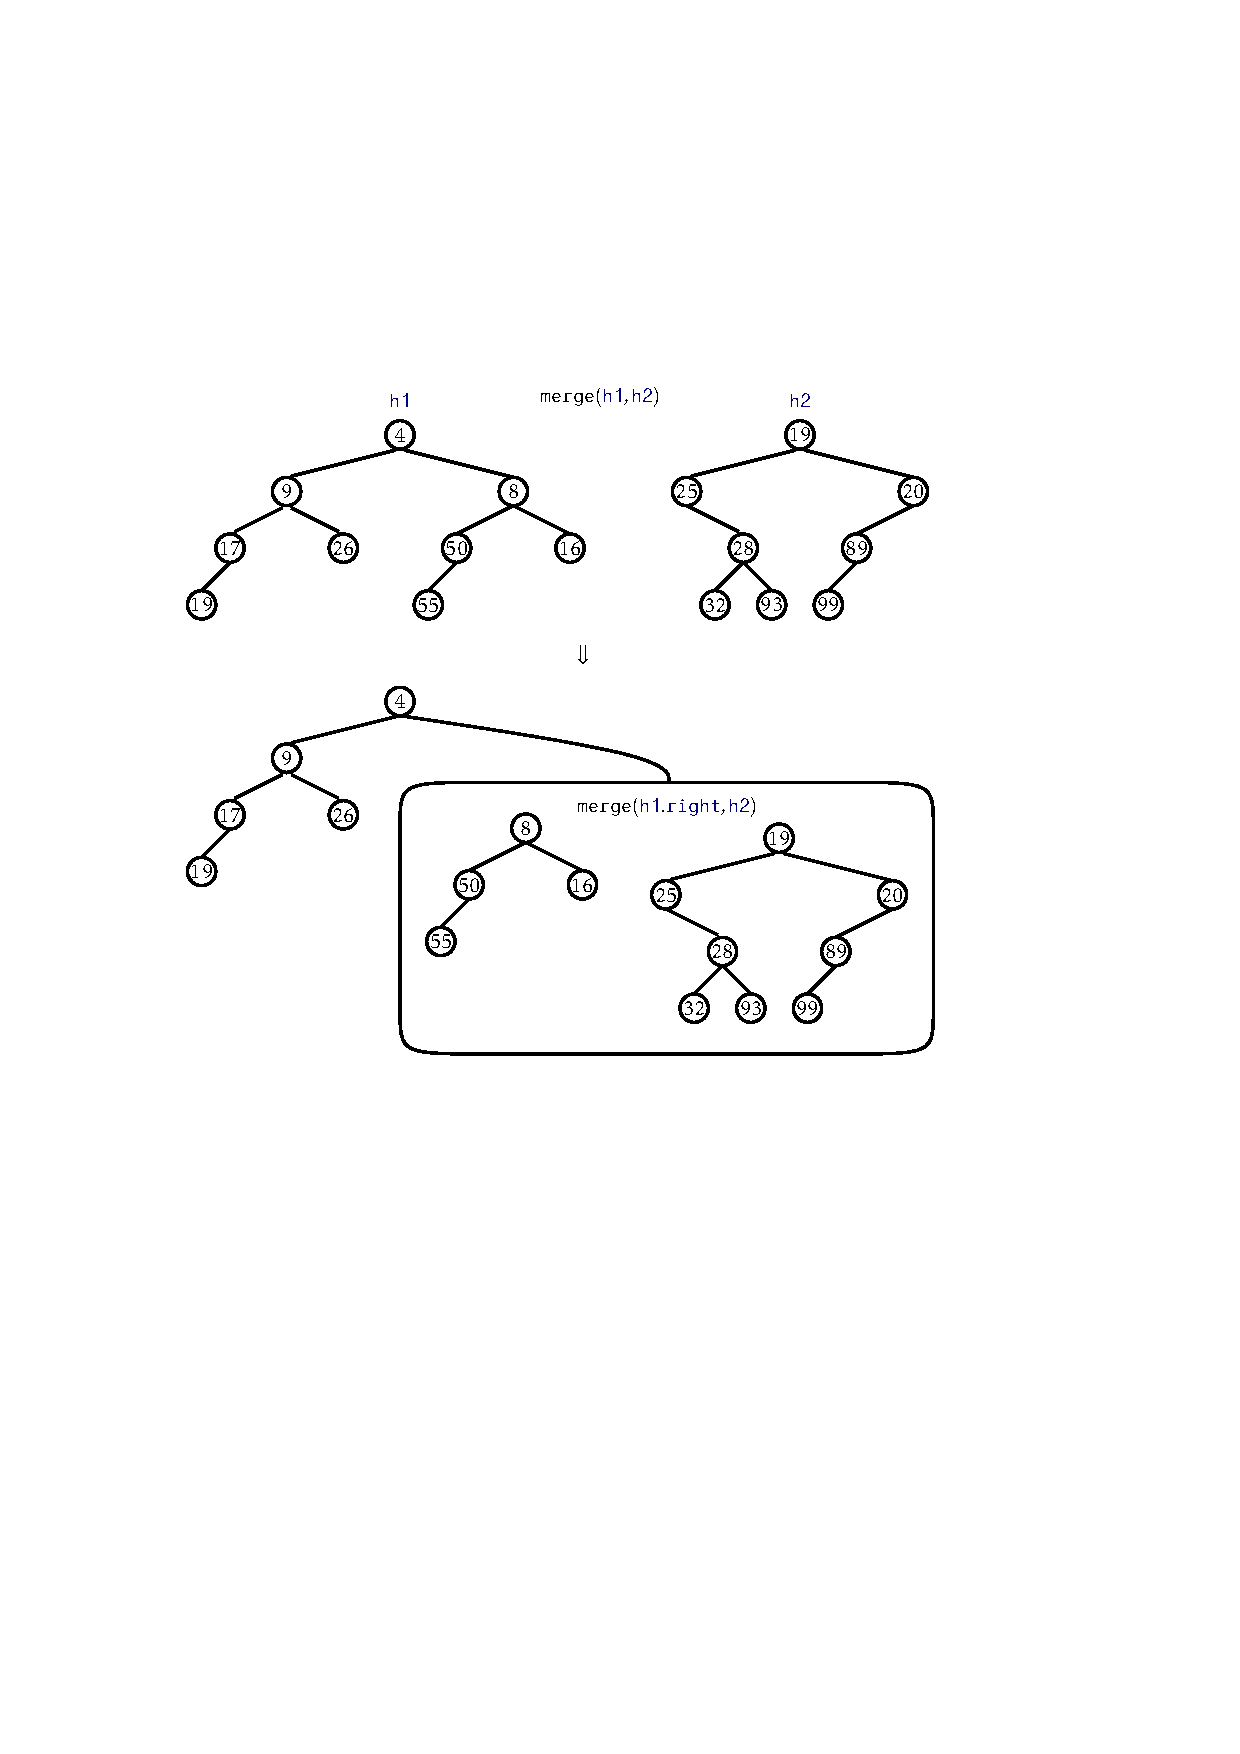
\includegraphics[width=\ScaleIfNeeded]{figs/meldable-merge}}
  \caption[Mesclando em uma MeldableHeap]{A mesclagem de #h1# e #h2# é feita mesclando #h2# com um dos #h1.left# ou #h1.right#.}
  \figlabel{meldable-merge}
\end{figure}

Na próxima seção, mostramos que #merge(h1,h2)# é executado em um tempo esperado de $O(\log #n#)$, onde #n# é o número total de elementos em #h1# e #h2#.

Com o acesso a uma operação #merge(h1,h2)#, a operação #add(x)# é fácil. Criamos um novo nó #u# contendo #x# e depois mesclamos #u# com a raiz do heap:
\codeimport{ods/MeldableHeap.add(x)}
Isto leva um tempo esperado de $O(\log (#n#+1)) = O(\log #n#)$.

A operação #remove()# é igualmente fácil. O nó que queremos remover é a raiz, então apenas mesclamos seus dois filhos e fazemos a raiz ser o resultado:

\codeimport{ods/MeldableHeap.remove()}
Novamente, isto leva um tempo esperado de $O(\log #n#)$.

Além disso, uma #MeldableHeap# pode implementar muitas outras operações em um tempo esperado de $O(\log #n#)$, incluindo:
\begin{itemize}
\item #remove(u)#: remove o nó #u# (e sua chave #u.x#) do heap.
\item #absorb(h)#: adicione todos os elementos da #MeldableHeap# #h# a este heap, esvaziando #h# no processo.
\end{itemize}
Cada uma dessas operações pode ser implementada usando um número constante de operações de #merge(h1,h2)#, cada uma levando um  tempo esperado de $O(\log #n#)$.

\subsection{Análise de #merge(h1,h2)#}

A análise de #merge(h1,h2)# é baseada na análise de um passeio aleatório em uma árvore binária. Um \emph{passeio aleatório} em uma árvore binária começa na raiz da árvore. Em cada passo da caminhada aleatória, uma moeda é lançada e, dependendo do resultado desse sorteio, a caminhada prossegue para a esquerda ou para o filho direito do nó atual. A caminhada termina quando cai da árvore (o nó atual se torna #nil#).

O seguinte lema é um tanto notável porque não depende de forma alguma da forma da árvore binária:

\begin{lem}\lemlabel{tree-random-walk}
	O comprimento esperado de um passeio aleatório em uma árvore binária com #n# nós é no máximo #\log (n+1)#.
\end{lem}

\begin{proof}
	A prova é por indução em #n#. No caso base, $#n#=0$ e a caminhada tem comprimento $0=\log (#n#+1)$. Suponha agora que o resultado seja verdadeiro para todos os inteiros não negativos $#n#'< #n#$.

Faça $#n#_1$ indicar o tamanho da subárvore esquerda da raiz, de modo que $#n#_2=#n#-#n#_1-1$ seja o tamanho da subárvore direita da raiz.

 Começando na raiz, a caminhada dá um passo e depois continua em uma subárvore de tamanho $#n#_1$ ou $#n#_2$. Pela nossa hipótese indutiva, a duração esperada da caminhada é então
\[
    \E[W] = 1 + \frac{1}{2}\log (#n#_1+1) + \frac{1}{2}\log (#n#_2+1)  \enspace , 
\] 
já que cada um de $#n#_1$ e $#n#_2$ é menor que $#n#$. Como $\log$ é uma função côncava, $\E[W]$ é maximizado quando $#n#_1=#n#_2=(#n#-1)/2$.
%To maximize this,
%over all choices of $#n#_1\in[0,#n#-1]$, we take the derivative and obtain
%\[
%    (\E[W])' = \frac{1}{2}(c/#n#_1 - c/(#n#-#n#_1-1)) \enspace , 
%\]
%which is equal to 0 when $#n#_1 = (#n#-1)/2$.  We can establish that
%this is a maximum fairly easily, so
Portanto, o número esperado de passos feitos pelo passeio aleatório é
\begin{align*}
    \E[W] 
    & = 1 + \frac{1}{2}\log (#n#_1+1) + \frac{1}{2}\log (#n#_2+1) \\
   & \le  1 + \log ((#n#-1)/2+1) \\
   & =  1 + \log ((#n#+1)/2) \\
   & =  \log (#n#+1)  \enspace . \qedhere 
\end{align*}
\end{proof}

Fazemos uma rápida digressão para observar que, para os leitores que conhecem um pouco da teoria da informação, a prova de \lemref{tree-random-walk} pode ser expressa em termos de entropia.


\begin{proof}[Prova Teórica de Informação de  \lemref{tree-random-walk}]
	Faça $d_i$ indicar a profundidade do $i$-ésimo nó externo e lembre-se de que uma árvore binária com #n# nós possui #n+1# nós externos. A probabilidade de o passeio aleatório atingir o $i$-ésimo nó externo é exatamente $p_i=1/2^{d_i}$, então o comprimento esperado do passeio aleatório é dado por
\[
   H=\sum_{i=0}^{#n#} p_id_i
    =\sum_{i=0}^{#n#} p_i\log\left(2^{d_i}\right)
    = \sum_{i=0}^{#n#}p_i\log({1/p_i})
\]
O lado direito desta equação é facilmente reconhecível como a
entropia de uma distribuição de probabilidade sobre $#n#+1$ elementos. Um fato básico sobre a entropia de uma distribuição sobre $#n#+1$ elementos é que ela não excede $\log(#n#+1)$, o que comprova o lema.
\end{proof}

Com este resultado em caminhadas aleatórias, agora podemos provar facilmente que o tempo de execução da operação #merge(h1,h2)# é $O(\log #n#)$.

\begin{lem}
	Se #h1# e #h2# forem as raízes de dois heaps contendo $#n#_1$ e $#n#_2$ nós, respectivamente, então o tempo de execução esperado de #merge(h1,h2)# é no máximo $O(\log #n#)$, onde $#n#=#n#_1+#n#_2$,
\end{lem}

\begin{proof}
	Cada etapa do algoritmo de mesclagem leva um passo de uma caminhada aleatória, na heap com raiz em #h1# ou na heap com raiz em #h2#.
  %, depending on whether $#h1.x# < #h2.x#$ or not.
  O algoritmo termina quando qualquer um desses dois caminhos aleatórios caírem de sua árvore correspondente (quando $#h1#=#null#$ ou $#h2#=#null#$).
  Portanto, o número esperado de passos executados pelo algoritmo de mesclagem é no máximo
  \[
     \log (#n#_1+1) + \log (#n#_2+1) \le 2\log #n# \enspace . \qedhere
  \]
\end{proof}

\subsection{Resumo}

O seguinte teorema resume o desempenho de uma #MeldableHeap#:

\begin{thm}\thmlabel{meldableheap}
	Uma #MeldableHeap# implementa a interface #Fila# (de prioridade).
	Uma #MeldableHeap# suporta as operações #add(x)# e #remove()#
	em um tempo esperado de $O(\log #n#)$  por operação.
\end{thm}

\section{Discussão e Exercícios}

A representação implícita de uma árvore binária completa como um array, ou lista, parece ter sido proposta pela primeira vez por Eytzinger \cite{e1590}.
Ele usou essa representação em livros contendo árvores genealógicas de pedigree 
\index{pedigree family tree}%
de famílias nobres. A estrutura de dados #BinaryHeap# descrita aqui foi introduzida pela primeira vez por Williams \cite{w64}.

A estrutura de dados #MeldableHeap# aleatória descrita aqui aparece
primeiramente proposta por Gambin e Malinowski \cite{gm98}.
Outras implementações de meldable heap existem, incluindo heaps de esquerda \cite[Seção~5.3.2]{c72,k97v3},
\index{leftist heap}%
\index{heap!leftist}%
heaps binomiais \cite{v78},
\index{binomial heap}%
\index{heap!binomial}%
heaps de Fibonacci \cite{ft87}, 
\index{Fibonacci heap}%
\index{heap!Fibonacci}%
heaps emparelhadas \cite{fsst86},\
\index{pairing heap}%
\index{heap!pairing}%
 e heaps inclinadas \cite{st83}, 
\index{skew heap}%
\index{heap!skew}%
embora nenhum desses seja tão simples quanto a estrutura #MeldableHeap#.

Algumas das estruturas acima também suportam uma operação\\ #decreaseKey(u,y)#
\index{decreaseKey@#decreaseKey(u,y)#}%
em que o valor armazenado no nó #u# é reduzido para #y#. (É uma
pré-condição que $#y#\le#u.x#$.) Na maioria das estruturas anteriores, esta operação pode ser suportada em um tempo $O(\log #n#)$ removendo o nó #u# e adicionando #y#. No entanto, algumas dessas estruturas podem implementar #decreaseKey(u,y)# com mais eficiência. Em particular, #decreaseKey(u,y)# leva um tempo amortizado de $O(1)$ nas heaps de Fibonacci e um tempo amortizado de $O(\log\log #n#)$  numa versão especial de heaps de emparelhamento \cite{e09}.
Essa operação #decreaseKey(u,y)# mais eficiente tem aplicações para
acelerar vários algoritmos gráficos, incluindo o algoritmo de caminho mais curto de Dijkstra \cite{ft87}.

\begin{exc}
	Ilustre a adição dos valores 7 e depois 3 ao #BinaryHeap# mostrado no final de \figref{heap-insert}.
\end{exc}

\begin{exc}
	Ilustre a remoção dos próximos dois valores (6 e 8) na #BinaryHeap# mostrada no final de \figref{heap-remove}.
\end{exc}

\begin{exc}
	Implemente o método #remove(i)#, que remove o valor armazenado em
	#a[i]# em #BinaryHeap#. Este método deve ser executado em um tempo $O(\log #n#)$.
	Em seguida, explique por que esse método provavelmente não será útil.
\end{exc}

\begin{exc}\exclabel{general-eytzinger}
  \index{tree!$d$-ary}%
  Uma árvore $d$-aria é uma generalização de uma árvore binária na qual cada nó interno possui $d$ filhos. Usando o método de Eytzinger também é possível representar árvores completas de $d$-aria usando arrays. Trabalhe as equações que, dado um índice #i#, determinam o índice do pai de #i# e cada um dos $d$ filhos de #i# nesta representação.
\end{exc}

\begin{exc}
  \index{DaryHeap@#DaryHeap#}%
  Usando o que você aprendeu em \excref{general-eytzinger}, projete e
  implemente um \emph{#DaryHeap#}, a generalização $d$-aria de um
  #BinaryHeap#. Analise os tempos de execução de operações em #DaryHeap# e teste o desempenho de sua implementação #DaryHeap# em relação à implementação #BinaryHeap# fornecida aqui.
\end{exc}



\begin{exc}
	Ilustre a adição dos valores 17 e 82 na #MeldableHeap# #h1# mostrada em \figref{meldable-merge}. Use uma moeda para simular um bit aleatório quando necessário.
\end{exc}

\begin{exc}
	Ilustre a remoção dos próximos dois valores (4 e 8) no #MeldableHeap# #h1# mostrado em \figref{meldable-merge}. Use uma moeda para simular um bit aleatório quando necessário.
\end{exc}

\begin{exc}
  Implemente o método #remove(u)# que remove o nó #u# de uma #MeldableHeap#. Estemétodo deve executar em um tempo esperado de $O(\log #n#)$.
\end{exc}

\begin{exc}
  Mostre como encontrar o segundo menor valor em uma #BinaryHeap#  
  ou #MeldableHeap# em um tempo constante
\end{exc}

\begin{exc}
	Mostre como encontrar o $k$-ésimo menor valor em uma #BinaryHeap# ou	#MeldableHeap# em um tempo $O(k\log k)$. (Dica: usar uma outra heap pode ajudar.)
\end{exc}

\begin{exc}
	Suponha que você tenha #k# listas ordenadas com um tamanho total de #n#. Utilizando uma heap, mostre como fundi-las em uma única lista ordenada em um tempo $O(n\log	k)$. (Dica: Começar com o caso $k=2$ pode ser instrutivo.)
\end{exc}








